% Set a sane document class, 10pt font, and a report template
\documentclass[a4paper,10pt]{report}


% Import used packages
\usepackage{graphicx}
\usepackage{hyperref}
\usepackage[margin=2.5cm]{geometry}
\usepackage{listings}
\usepackage{longtable}
\usepackage{lscape}

% Bibliographies
\usepackage{biblatex}
\bibliography{slr-scbw/bib/bib}
\bibliography{bibliography}

% Use UTF-8
%\usepackage[utf8x]{inputenc}

\def \authors {Ken Børge Viktil and Martin Tobias Holmedahl Sandsmark}
\def \papertitle {A cognitive architecture for playing Starcraft: Brood War}

% Meta-information for the PDF
\hypersetup{
pdfauthor = \authors,
pdftitle = \papertitle,
pdfsubject = {Pre-project for IDI},
pdfkeywords = {project, cognitive, architecture, starcraft, artificial
    intelligence},
pdfcreator = {LaTeX with hyperref package},
pdfproducer = {pdflatex}}

%opening
\title{\papertitle}
\author{\authors}

\begin{document}


\maketitle

\begin{abstract}
We present an overview of existing research into the use of cognitive models
for artificial intelligences, the game Starcraft: Broodwar, and research into
architectures for artificial intelligence for playing the game.
\end{abstract}

\tableofcontents

\chapter{Introduction}

\section{Background and motivation}
\subsection{StarCraft: Brood War and BWAPI}
StarCraft is one of the most popular real time strategy games in the world. It
is developed by Blizzard Entertainment, and in 1998 they released the expansion
pack Brood War which they had developed together with Saffire.

Since its release it has been widely played in professional tournaments, as
well as been used extensively in research on artificial intelligence, partly
thanks to the BWAPI project which is a project to develop and maintain an API
for developing artificial intelligences that play the game. In addition, this
API is the basis for a yearly competition where people can submit artificial
intelligences developed with this API. This has led to a fairly large number of
AIs being developed, of various degrees of complexity and novelty.

Most architectures are fairly straight-forward and rule-based, with some
novel research into using multi-agent systems which seems to be fairly
successful.

\subsection{Cognitive architectures}
One area that haven't been as well explored in relation to RTSes in general and
StarCraft in particular, is cognitive architectures, architectures inspired by
mental processes. There has been some research done into implementing cognitive
models for use in first-person shooter games, but not into real-time strategy
games. It would seem intuitive that real-time strategy games, which have been
considered a relatively hard problem to solve in a human-like fashion, would
benefit from using models based on our understanding of human cognition.


\section{Goals and Research Question}
We want to explore the use of a cognitive architecture for the use in an AI for
StarCraft: Brood War.

Our research goal is as follows:
\begin{quote}
 ``Develop a novel AI Architecture for StarCraft: Brood War.''
\end{quote}


\section{Contributions}
The following individuals has contributed to the work presented in this report.

\begin{enumerate}
 \item Helge Langseth
 \item Anders Kofod-Petersen
 \item Pauline Haddow
 \item Adam Heinermann
\end{enumerate}


\section{Research Method}
We herped the derp.


\section{Structure}
This paper is structured in four chapters; the introductory chapter you're
currently reading, a chapter on the theory and background for the research, a
chapter on the research results themselves and finally a chapter with the
evaluation of the research and a conclusion.
%!TEX root = main.tex

\chapter{Theory}
\section{Starcraft}

\begin{figure}[h!tb]
\centering
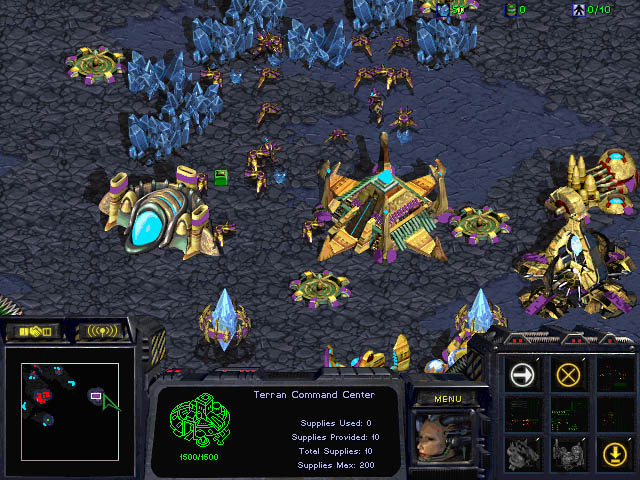
\includegraphics[scale=0.5]{graphics/scbw.jpg}
\caption{Star Craft Brood War \cite{test}}
\label{fig:scbwIntro}
\end{figure}
StarCraft is on the surface a very simple game, it has only three different playable races, a
handful of different buildings and units, and relatively simple to comprehend
goals. But once you start analyzing the game, the reality is quite different. The brood war expansion pack was released back in 1998, and has been played at a high level since that and all the way up to today. And the meta game has evolved during the entire lifespan of the game and is still changing today with new tactics showing up from tournament to tournament.
\cite{blizzardstarcraft}

When playing at a really high level you are working with really small windows of opportunity, often called timings. And it is these timings that enable a game with what should in theory be simple elements to have such complex and evolving strategies. 


\section{Artificial Intelligences for StarCraft}
There have been a handful of relatively successful AIs for StarCraft.

\subsection{In-game AI}
The in-game AI is considered not very good.

\subsection{Berkeley Overmind}
This is considered one of the best AIs, not perhaps because it is very complex,
but because it has a solid ``cheese'' and has been well-tweaked.


\section{Architectures}
\subsection{General architectures}
\subsection{Cognitive Architectures}
\paragraph{Global Workspace Theory}
\paragraph{Cognitive Models in game AIs}
\citeSLR{Arrabales2009}

\chapter{Results}

\section{Architecture}
We chose a cognitive architecture partially inspired by the CERA-CRANIUM
architecture.

\section{Experimental plan and setup}
We played a lot of games.


\section{Experimental results}
We won a lot of games.
\chapter{Evaluation}
\section{Evaluation of results}
The results were good.


\section{Summary}
The good was great.


\section{Discussion}


\section{Contributions}
We wrote most stuff ourselves, but we used blah and blergh.


\section{Impact}
We believe that this will change the human condition.


\section{Future work}
Skynet.

% Appendix
\chapter{Appendix 1}
\label{appendix:slrreport}
\section{Introduction}
%!TEX root = main.tex

\chapter{Introduction}

\section{Background and motivation}

\subsection{The Problem}
In 2003 Michael Buro published an article where he requested more artificial
intelligence research in the domain of real-time strategy
games.\cite{buro2003real} Before this, a lot of research was focused mainly on
turn based, real-time board games, like chess and checkers. A lot of
progress has been done in these fields to the point where they are now able to
beat top level human players in a real-time match. \cite{campbell2002deep} But
these games are both deterministic and fully observable, whereas real-time
strategy games usually are only partially deterministic and partially
observable, which makes for much more interesting problems.

In the wake Buro's call to arms more work has been invested in this area, and
several platforms for RTS research has been used. One platform that has been
used a lot is Wargus\cite{wargus}, a clone of Blizzard's Warcraft 2, where they
created a Lua-based AI scripting language for efficient artificial game-playing
agent creation. But this game had quite severe limitations on individual
management of units, so in recent years StarCraft: Brood War has been getting a
lot more attention as a platform for experimenting with game playing agents.
Several competitions are held each year where implemented AI agents can
compete with each other and measure their performance. But even though a lot has
happened with the field in recent years, Starcraft agents still have ways to go
before they can measure up to a human player.\cite{eisbotvsfong}.

Simply winning is however not always the goal, most game-playing artificial
intelligences are made to be realistic and engaging to compete with, so in many
situations simply playing well is not enough. According to Arrabales et
al \cite{arrabales2009gamechars} it is still more realistic and engaging to be
playing with other humans than with synthetic agents. So to attempt to lessen
this gap, it could be interesting to make synthetic agents play more human-like,
and to do this one would probably want to look into more biologically inspired
methods, for example inspired by cognitive architectures.

Cognitive architectures have proven to lead to human-like behaviour and choices
in both games\cite{arrabales2009gamechars} and general problem
solving\cite{franklin2003interacting}, and the logical conclusion therefore
seems to be to try to apply these models to StarCraft.

\subsection{StarCraft: Brood War and BWAPI}
StarCraft is one of the most popular real-time strategy games in the world. It
was developed by Blizzard Entertainment, and in 1998 they released the expansion
pack Brood War. The expansion pack included new maps, units and upgrades for
each of the races in the game.
 
Since its release it has been widely played in professional tournaments, as well
as been used extensively in research on artificial intelligence, thanks to the
BWAPI project which is a free software project aimed at developing and
maintaining an API, named BWAPI, for creating artificial intelligence modules
for Brood War. In addition, this API is the basis for several yearly
competitions where people can submit AI bots that will be pitted against other
bots to measure their relative performance. This has led to a large number of
AIs being developed of various degrees of complexity and novelty, both from
researchers and hobby developers. 

\subsection{The project}
In this project we will familiarize ourselves with the game StarCraft: Brood
War, and what challenges that presents when creating a computer program that
will play the game. We will identify the different aspects of a StarCraft game
that are important to solve in order to create a good game-playing agent, and
also look at how other researchers have solved these problems in their agents.
Ultimately we will select and define an architecture for our system that will
have an modular approach in order to support easier collaboration when
implementing the system, based on a cognitive model.

In order to get a good overview of existing solutions and map the current state
of the research into this field, we will perform a structured literature review.
This will give us a good overview of the theory behind the state of the art
when it comes to our research problem.

So our project is divided into three main parts:
\begin{enumerate}
  \item Identify the most important aspects of a StarCraft match.
  \item Research existing solution and theories, using a structured literature
review.
  \item Design an architecture for a modular StarCraft playing computer
program, based on a cognitive model.
\end{enumerate}

\section{Contributions}
For the structured literature review we collaborated with Magnus Sellereite
Fjell, Stian Veum M{\o}llersen, Tobias Laupsa Nilsen, J{\o}rgen B{\o}e Svendsen,
Espen Auran Rathe, Aleksander Lun{\o}e Waage, {\O}ystein Samuelsen, Finn Robin
K{\aa}veland Hansen, Dag-{\O}yvind Tornes and Jan Eriksson.

We are also grateful for the feedback and cooperation with everyone on the
\#BWAPI IRC channel on QuakeNet, and especially Adam Heinermann who is also a
lead developer on the BWAPI project.

We would also like to thank our supervisors; Helge Langseth, Anders
Kofod-Petersen and Pauline Haddow.

\section{Report Structure}
This report is structured into four chapters:
\begin{itemize}
\item Chapter 1: \textbf{Introduction} \\
This chapter describes the motivation and goal of the project as well as who contributed and the general structure of the report.
\item Chapter 2: \textbf{Theory} \\
This chapter is threefold. First it presents some theory on StarCraft in
general, how the most important mechanics works and the difference between the
available races. Then we go over the state of the art when it comes to agents
who play StarCraft, both how the problems they solve are partitioned, as well
as how some of the most important agents today are architected. Lastly we go
over some background on the current state of cognitive research and models
utilizing this.
\item Chapter 3: \textbf{Results} \\
Here we present our results; our novel architecture for an agent for playing
StarCraft: Brood War based on the cognitive models we explored earlier.
\item Chapter 4: \textbf{Evaluation} \\
Here we summarize and evaluate the work presented in this report.




\end{itemize}

\section{Structured Literature Review}
\input{slr-scbw/sections/about_slr}

\section{Protocol and Procedure}
\input{slr-scbw/sections/protocol}

\section{Search Engines and Search Strings}
\input{slr-scbw/sections/search_engines}

\section{Search Results}
\input{slr-scbw/sections/search_results}

\clearpage
\bibliographystyle{unsrt}
\bibliography{slr-scbw/bib/bib}

\printbibliography

\end{document}
